\ihead{Florian Greistorfer}
\chapter{Webserver und Client}

\begin{figure}[H]
	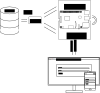
\includegraphics[width=1\textwidth]{Bilder/SVGS/Communication}
	\caption{Kommunikationen innerhalb des Projekts}
	\label{kommunikation}
\end{figure}

\section{Begriffserklärungen}
\label{sec:begriffserklaerung}

\subsection{Server}
\label{sec:begrr-server}
Ein Programm, das Zugriff auf eine Ressource oder einen Dienst in einem Netzwerk ermöglicht

\subsection{Client}
\label{sec:begrr-client}
Ein Programm, das auf einen Server zugreift

\section{Anforderungen}
\label{sec:anforderungen}

\subsection{Webserver}
\label{sec:anf-server}
Auf der Katzenfütterungsanlage läuft ein Webserver, der es ermöglicht, dass der Benutzer das Gerät über das Internet erreichen kann. Hauptaufgaben des Servers sind dabei, Daten bereitzustellen, zu verarbeiten und zu speichern und den Webclient zur Verfügung zu stellen.

\subsection{Client}
\label{sec:anf-client}
Der Client soll dem Benutzer ermöglichen, die Katzenfütterungsanlage über einen Webbrowser zu steuern. Ein Benutzername und ein Passwort sind erforderlich, damit man das Gerät bedienen kann. Das Design soll eindeutig und übersichtlich gehalten sein. Auf der Startseite sollen die eingestellten Fütterungszeiten und eine allgemeine Übersicht zu sehen sein. Über eine Navigationsleiste sollen die weiteren Seiten erreichbar sein:

\begin{itemize}
\item[•]Fütterrungszeiten
\item[•]Positionsinfo
\item[•]Geräteinfo
\item[•]Update
\end{itemize}

\section{Voruntersuchung}
\label{sec:voruntersuchung}

\subsection{HTTP/HTTPS}
\label{sec:vor-http}
Das \ac{HTTP}\footnote{Weitere Informationen zu \ac{HTTP} unter \url{https://developer.mozilla.org/de/docs/Web/HTTP}} ist der Kommunikationsstandard auf dem das Internet basiert. Eine HTTP Session wird über eine Anfrage über das \ac{TCP} an einen Server auf den Port 80 initiiert. Der Server, der auf diesem Port auf eine Anfrage wartet, sendet eine Statusmeldung wie z.B. \inlinecode{bash}{HTTP/1.1 200 OK} und eventuell eine eigene Nachricht zurück. Diese Nachricht ist meist die angeforderte Resource oder eine Fehlermeldung. \ac{HTTPS} ist die verschlüsselte Version von \ac{HTTP}. Die meist gebrauchten Anfragen sind:

\begin{itemize}
\item[•] \textbf{GET}: Fordert eine Repräsentation der Ressource an. Ein GET Request darf nur Daten abfragen und darf keinen anderen Einfluss haben.
\item[•] \textbf{PUT}: Fordert das Speichern der Daten, die sich im Request-Body befinden, an. Wenn bereits eine Ressource an der angegebenen \ac{URI} existiert, so wird diese aktualisiert, sonst wird die Resource erstellt.
\item[•] \textbf{POST}: Fordert das Speichern der Daten, die sich im Request-Body befinden, unter der angegebenen \ac{URI} an. 
\item[•] \textbf{DELETE}: Fordert das Löschen der Ressource unter der angegebenen \ac{URI} an.
\end{itemize}

\subsubsection{HTTP Status Codes}
\label{sec:http-status-codes}
\begin{itemize}
\item[•] \textbf{1xx}: Information
\item[•] \textbf{2xx}: Erfolg
\item[•] \textbf{3xx}: Umleitung
\item[•] \textbf{4xx}: Client Fehler
\item[•] \textbf{5xx}: Server Fehler
\end{itemize}

\subsection{JavaScript}
\label{sec:vor-js}
JavaScript ist die Programmiersprache des Internets. Jeder herkömmliche Browser ist in der Lage, JavaScript auszuführen. Mit JavaScript ist es möglich, das Aussehen einer Webseite während der Laufzeit zu ändern, Dinge zu entfernen, hinzuzufügen und zu animieren. JavaScript ist heute eine objektorientierte Sprache. Es hebt sich von anderen Sprachen vor allem dadurch ab, dass die Datentypen von Variable nicht fix sind. Das bedeutet, wenn eine Variable den Datentyp \textit{number} hat und es wird ein String angehängt, verändert sich der Datentyp automatisch auf \textit{string}. JavaScript kann nur in einem Thread laufen, das bedeutet, es gibt kein echtes Multithreading. Damit etwas Ähnliches erzielt werden kann, gibt es die Möglichkeit von Callback Methoden. Diese werden ausgeführt, sobald etwas vorher abgeschlossen wurde. Damit ist es möglich, Dinge, die länger brauchen, im ''Hintergrund'' laufen zu lassen\footnote{Mehr Information zu Callbacks, Promises und JavaScript unter \url{https://www.w3schools.com/js/default.asp}}.

\subsection{TypeScript}
\label{sec:vor-ts}
TypeScript ist eine, von Microsoft entwickelte, Weiterentwicklung von JavaScript. Das bedeutet, jeder gültige JavaScript Code ist auch ein gültiger TypeScript Code. TypeScript wird vom TypeScript Compiler in sauberes JavaScript übersetzt. TypeScript ist sehr gut für größere Anwendungen geeignet. Typescript hat strenge Datentypen, Klassen und Vererbung. Die Datentypen von TypeScript sind:

\begin{itemize}
\item[•] \textbf{string}: eine Unicode codierte Zeichenkette, von JavaScript übernommen
\item[•] \textbf{number}: eine vorzeichenbehaftete Gleitkommazahl, kann auch hexadezimal, octal oder binär sein, von JavaScript übernommen
\item[•] \textbf{boolean}: true oder false, von JavaScript übernommen
\item[•] \textbf{array}: eine Liste von Elementen des gleichen Datentyps, von JavaScript übernommen
\item[•] \textbf{tuple}: eine Liste von Elementen unterschiedlichen Datentyps, deren Anzahl bekannt ist
\item[•] \textbf{enum}: eine Möglichkeit, numerischen Werten Namen zu geben
\item[•] \textbf{any}: Datentyp unbekannt, wird behandelt wie in JavaScript
\item[•] \textbf{void}: kein Datentyp, meist Rückgabewert bei Funktionen
\item[•] \textbf{null}: leerer Wert, kann allen anderen zugewiesen werden, von JavaScript übernommen
\item[•] \textbf{undefined}: kein Wert, kann allen anderen zugewiesen werden, von JavaScript übernommen
\item[•] \textbf{never}: wenn ein Wert niemals auftreten kann z.B. eine Funktion die immer einen Fehler produziert
\end{itemize}

Damit JavaScript Module von TypeScript verwendet werden können, benötigen sie sogenannte Type Annotations. Diese können bei den meisten bekannteren Modulen über den \ac{npm} installiert werden. Diese Pakete haben den Namenspräfix \textit{@types/}, das bedeutet, dass zum Beispiel die Type Annotations des Express Moduls über \inlinecode{bash}{npm install --save-dev @types/express} installiert werden können. Sollten keine Type Annotations für ein Modul vorhanden sein, muss man diese selbst erstellen.

\subsection{HTML}
\label{sec:vor-html}
\ac{HTML} ist eine Markup Language, zu Deutsch Auszeichnungssprache, dies bedeutet, sie ist keine Programmiersprache, sondern beinhaltet nur Informationen, wie etwas dargestellt werden soll. Eine \ac{HTML} Datei ist rein textuell und wird erst durch ein Programm, z.B. einen Browser, formatiert dargestellt. \ac{HTML} ist der Standard für alle Websites im Internet. Eine \ac{HTML} Datei kann aus drei Teilen bestehen. Dem eigentlichem \ac{HTML}, JavaScript und Styles. JavaScript und Styles können zur besseren Übersicht in eigenen Dateien ausgelagert werden.

\subsection{CSS}
\ac{CSS} sind die Style Dateien einer Website. In einer \ac{CSS} Datei steht, wie ein \ac{HTML} Element aussieht. Mithilfe von Styles kann z.B. die Farbe, Größe, Platzierung, Schriftart und vieles mehr eines Elementes bestimmt werden. Da das Design in eine eigene Datei ausgelagert wurde, muss es eine Zuweisung zwischen \ac{CSS} und \ac{HTML} geben. Dafür gibt es drei Arten. Entweder man weist es jedem Element dieses Typs zu, nur einem Element mit einer bestimmten ID oder jedem Element einer bestimmten Klasse. Mit dem Schlüsselwort \inlinecode{css}{!important} kann man bestimmen, welcher Style bevorzugt genommen wird, wenn eine Doppelbelegung existiert.

\begin{lstlisting}[caption=Zuweisen von Design an HTML,style=css,label=CSS-Beispiel]
body { // Zuweisung an alle Elemente eines Typs
	background-color: cyan;
}

#title { // Zuweisung an ein Element mit einer ID
	color: red;
}

.text { // Zuweisung an alle Elemente einer Klasse
	border: 1px solid black;
}
\end{lstlisting}


\subsection{DOM}
\label{sec:vor-dom}
Das \ac{DOM} ist die Objektrepräsentation des \ac{HTML} Dokuments. Durch das \ac{DOM} kann eine JavaScript Anwendung \ac{HTML} Elemente ändern, entfernen oder hinzufügen, sowie \ac{HTML} Attribute ändern, entfernen oder hinzufügen und \ac{CSS} Styles ändern. Das \ac{DOM} wird vom Browser beim Laden der Website erstellt. 

\subsection{Node.js}
\label{sec:vor-node}
Node.js ist eine Laufzeitumgebung, die es ermöglicht, dass Javascript direkt auf einem Rechner ausgeführt werden kann. Node.js kommt mit dem \ac{npm}. Mithilfe diesem Tools ist es möglich, Module zu installieren, updaten, löschen und veröffentlichen. Diese Module werden im Ordner \textit{/node\_modules} installiert und in der Datei \textit{package.json} unter \textit{dependencies}, oder mit der option \inlinecode{bash}{--save-dev} unter \textit{dev-dependencies} eingetragen. Ein neues Projekt erstellt man mit \inlinecode{bash}{npm init}. Dieses Tool erstellt die Datei \textit{package.json}, in der alle Abhängigkeiten und Informationen über das Projekt stehen. Wenn man ein Projekt kopiert, braucht man den \textit{/node\_modules} Ordner nicht mitkopieren. Man muss nur im Zielordner einmal \inlinecode{bash}{npm install} aufrufen.

\subsection{express}
\label{sec:vor-express}
Express ist ein Javascript Modul, das auf dem Node.js Modul \textit{http} bzw \textit{https} aufbaut. In diesen Modulen ist bereits alles enthalten, was benötigt wird, um einen Webserver zu programmieren. Express nimmt uns die meiste Arbeit ab und bietet viele weitere Möglichkeiten\footnote{Weitere Information zu express unter \url{https://expressjs.com/}}.

\subsection{JSON}
\label{sec:vor-json}
\ac{JSON} ist die Textrepräsentation eines JavaScript Objekts\footnote{Weitere Informationen zu \ac{JSON} unter \url{https://www.json.org/}}. Die möglichen Datentypen sind:

\begin{itemize}
\item[•] \textbf{string}: 0 oder mehrere unicode Zeichen innerhalb Doppelhochkommas
\item[•] \textbf{boolean}: true oder false
\item[•] \textbf{number}: Eine vorzeichenbehaftete Zahl, die auch die E Notation unterstützt z.B. 0.2E4 (=2000)
\item[•] \textbf{Array}: Eine geordnete Liste von 0 oder mehreren Werten innerhalb eckiger Klammern, Elemente sind getrennt durch Kommas.
\item[•] \textbf{Object}: Eine ungeordnete Sammlung von Name-Wert-Paaren, wo die Namen, die auch Keys genannt werden, Strings sind. Jeder Key sollte eindeutig sein. Befindet sich innerhalb geschwungener Klammern. Paare sind durch Komma getrennt
\item[•] \textbf{null}: Ein leerer Wert
\end{itemize}

\begin{lstlisting}[style=JSON,caption=\ac{JSON} Beispiel]
{
	"Object": {	
		"string": "name",
		"number": 10E5,
		"boolean": true,
		"Array": [
			{
				"string": "wert",
				"number": 1
			},
			{
				"string": "wert",
				"number": 2
			}
		]
	}
}
\end{lstlisting}

\subsection{JSON Web Token}
\label{sec:vor-jwt}
\ac{JWT} ist ein JSON-basierter offener Standard für das Erstellen von Access Tokens. Mithilfe eines \ac{JWT} kann ein Client sich ausweisen. Ein \ac{JWT} wird vom Server entweder mit einem Secret oder seinem privaten Schlüssel signiert. Dadurch können Server und Client überprüfen, ob der Token legitim ist. Ein \ac{JWT} besteht aus drei Teilen: dem Header, der Payload und der Signature. Im Header steht der fürs Verschlüsseln der Signatur benutzte Algorithmus z.B: \inlinecode{JSON}{\{"alg":"RS256","typ":"JWT"\}}. Im Payload stehen die Daten, die entweder den Client ausweisen oder ähnliche Information. Beispiel: \inlinecode{JSON}{\{"user": "cat", "iat": 1520875121, "exp": 1520911121\}} \textit{iat} bedeutet \textit{issued at} und sagt aus, wann der Token generiert wurde. In der Signature stehen der Key, der unsignierte Token, das ist der Header und die Payload Base64 codiert, und die Signatur. Alle drei Teile werden Base64 codiert und mittels Punkt voneinander getrennt.

\subsection{MongoDB}
\label{sec:vor-mongo}
MongoDB ist eine schemenlose Datenbank. Schemenlos bedeutet, dass die Datenbank im Vergleich zu schemenbehafteten Datenbanken keine klare Strukturierung benötigt. Einer schemenlosen Datenbank kann man einfach Daten geben und wieder abfragen. Eine schemenbehaftete Datenbank ist in Zeilen und Spalten unterteilt. Diese müssen vorher feststehen. Da Raspian, das Betriebssystem vom Raspberry Pi, nur 32 Bit ist und MongoDB ab Version 3 nur mehr in 64 Bit erhältlich ist, mussten wir auf eine ältere Version wechseln. Die Verbindung der MongoDB Datenbank erfolgt über einen Driver. Der Driver muss mit der Datenbankversion übereinstimmen. MongoDB ist ein \ac{DBMS}. Das bedeutet, ein Server läuft auf dem Port 27017, über den alle Datenbanken im System erreichbar sind, beispielsweise ist die Datenbank \textit{fuettr} über \inlinecode{bash}{localhost:27017/fuettr} erreichbar. Eine Gruppe von Daten nennt man Collection. Zugriff auf die Datenbank erfolgt serverseitig wie folgt:

\begin{lstlisting}[caption=Verbinden mit dem \ac{DBMS},style=TS]
const dbServer = await mongodb.MongoClient.connect(url);
\end{lstlisting}

\begin{lstlisting}[caption=Auswählen der Datenbank,style=TS]
const dbFuettr = await dbServer.db('fuettr');
\end{lstlisting}

\begin{lstlisting}[caption=Auswählen der Collection,style=TS]
const collTimes = await dbFuettr.collection('data_times');
\end{lstlisting}

\begin{lstlisting}[caption=Auslesen aller Datensätze mit einem Identifier,style=TS]
const Times = await this._times.find({ identifier: 'Times' }).toArray();
\end{lstlisting}

\begin{lstlisting}[caption=Überschreiben eines Datensatzes mit einem Identifier,style=TS]
this._times.updateOne({ identifier: 'Times' }, { $set: times });
\end{lstlisting}

\subsection{Angular 2/4}
\label{sec:vor-angular}
Angular ist ein TypeScript Framework, das aus dem Javascript-Framework AngularJS weiterentwickelt wurde. Es wird von Google entwickelt. Angular ist gegliedert in Module. Die grobe Struktur wird in der Abbildung \ref{Angular Struktur} dargestellt\footnote{Genauere Informationen und Tutorials unter \url{https://angular.io/}}.

\begin{figure}[H]
      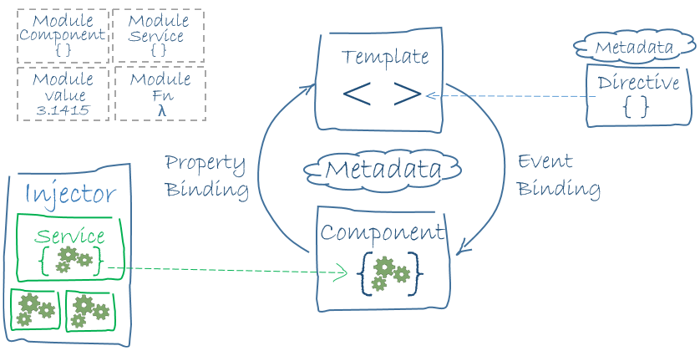
\includegraphics[width=1\textwidth]{Bilder/Greistorfer/Angular}
      \caption[Angular Struktur]{Angular Struktur\protect\footnotemark}
      \label{Angular Struktur}
\end{figure}

\footnotetext{\autoref{Angular Struktur} Quelle: \url{https://angular.io/guide/architecture\#whats-next} (besucht am 10.3.2018)}

\subsubsection{Modules}
\label{sec:ang-modules}
Jede Angular App ist in \textit{Module}s gegliedert. \textit{Module}s fassen meist ähnliche Funktionen zusammen. Jede App muss mindestens ein \textit{Module} enthalten. Dies heißt standardmäßig \textit{AppModule}. Ein \textit{Module} ist die größte Einheit einer Angular App.  Ein \textit{Module} kann folgende Komponenten beinhalten:

\begin{itemize}
\item[•]Services
\item[•]Andere Module
\item[•]View Classes
\begin{itemize}
\item[-]Components
\item[-]Directives
\item[-]Pipes
\end{itemize}
\end{itemize}

\subsubsection{Libraries}
\label{sec:ang-libraries}
Eine Angular Library ist ein Modul, das \textit{Modules} exportiert. Diese können von \textit{Components} und \textit{Modules} importiert werden. Der Name jeder Angular library beginnt mit \textit{@angular}. Angular libraries können mit dem \ac{npm} installiert werden.

\subsubsection{Components}
\label{sec:ang-components}
Ein \textit{Component} kontrolliert einen Teil des Bildschirms, den sogenannten \textit{view}. Die Logik des \textit{Component}s wird in einer Klasse definiert. Die Klasse interagiert mit dem \textit{view} durch eine \ac{API} von Eigenschaften und Methoden.

\paragraph*{Lifecycle Hooks}\mbox{}\\
Ein Lebenszyklus in Angular ist immer der Lebenszyklus des jeweiligen \textit{Components}. Ein \textit{Component} kann erstellt, verändert und zerstört werden. Zu jedem Stadium gibt es eine Methode, die automatisch je nach Stadium von Angular aufgerufen wird. Die am häufigsten verwendeten sind:

\begin{itemize}
\item[•] \textbf{OnInit()}: Wird aufgerufen, wenn der \textit{Component} erstellt wird. Die dazugehörige Methode ist \inlinecode{TS}{ngOnInit()}. Zeitaufwendige Operationen sollten anstatt im constructor hier aufgerufen werden, da das den Erzeugungsvorgang verlangsamen würde.
\item[•] \textbf{OnDestroy()}: Wird aufgerufen, wenn der \textit{Component} zerstört wird. Die dazugehörige Methode ist \inlinecode{TS}{ngOnDestroy()}. Hier sollten alle laufenden Prozesse wie Intervals und Callbacks beendet werden.
\item[•] \textbf{OnChanges()/DoCheck()}: Werden aufgerufen, wenn sich irgendetwas an der \textit{Component} ändert. Die dazugehörige Methoden sind \inlinecode{TS}{ngOnChanges()} und \inlinecode{TS}{ngDoCheck()}.
\end{itemize}

Alle Lifecycle Hooks müssen von der Klasse mit \inlinecode{TS}{implements} implementiert und von \textit{@angular/core} importiert werden.

\subsubsection{Templates}
\label{sec:ang-templates}
Das Aussehen des \textit{view}s wird in einem \textit{Template} definiert. Ein \textit{Template} ist eine \ac{HTML} Datei, mit Angular's Template Syntax. Das bedeutet, dass einige Zusatzbefehle vorkommen können. Beispiele hierfür sind:

\begin{itemize}
\item[•]*ngFor
\item[•]*ngIf
\item[•]\{\{variable\}\}
\item[•](click)
\item[•][variable]
\item[•]<app-route>
\end{itemize}

Die meisten Zusatzbefehle werden für \textit{Data Binding} verwendet.

\mbox{}
\begin{wrapfigure}{l}{0.5\textwidth}
\vspace{-50pt}
  \begin{center}
    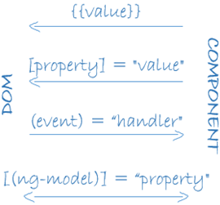
\includegraphics[width=0.4\textwidth]{Bilder/Greistorfer/databinding}
  \end{center}
  \caption[Angular Databinding]{Angular Databinding\protect\footnotemark}
  \label{Angular Databinding}
  \vspace{0pt}
\end{wrapfigure}
\vspace{-40pt}

\footnotetext{\autoref{Angular Databinding} Quelle: \url{https://angular.io/guide/architecture-components\#data-binding} (besucht am 10.3.2018)}

\subsubsection{Data binding}
\label{sec:ang-data-binding}
Ohne Framework wäre der Programmierer dafür verantwortlich sicherzustellen, dass Daten in \ac{HTML} Elemente geschrieben werden und dass auf Benutzerinteraktionen reagiert wird. Das ist aufwendig, fehleranfällig und schwer zu lesen. Angulars Lösung dafür nennt sich \textit{data binding}. Der Programmierer muss nur mehr im \ac{HTML} Template Angular mitteilen, wie die beiden Seiten verbunden werden sollen. In der Abbilung \ref{Angular Databinding} sind die vier möglichen Arten von \textit{data binding} dargestellt. Jede Art hat eine Richtung, vom \ac{DOM} zum \ac{DOM} oder in beide Richtungen.

\begin{itemize}
\item[•] \inlinecode{Html}{<span>\{\{variable\}\}</span>} Der Wert der Variable in den Klammern wird anstelle des Klammerausdrucks dargestellt. Wenn sich der Wert ändert, ändert sich auch der Wert im \ac{DOM}
\item[•] \inlinecode{Html}{<span [hidden]="hide"></span>} übergibt den Wert in der angegebenen Variable in das angegebene Attribut
\item[•] \inlinecode{Html}{<span (click)="clicked(\$event)"></span>} ruft die angegebene Methode auf, wenn das angegebene Event auftritt, in diesem Fall ein click-Event
\item[•] \inlinecode{Html}{<input [(ngModel)]="variable">} der Wert im Eingabefeld und in der Variable sind voneinander abhängig, ändert sich der eine, so ändert sich zugleich der andere zum gleichen Wert
\end{itemize}

\subsubsection{Services}
\label{sec:ang-services}
Services sind Klassen, die eine Aufgabe erfüllen, unabhängig von allem anderen. Sie werden vor allem verwendet, wenn eine Aufgabe etwas Zeit erfordert wie z.B. eine Serveranfrage. Services bieten auch die Möglichkeit, dass \textit{Components} Zugriff auf eine gemeinsame Variable haben, da Angular keine globalen Variablen hat. Services müssen vom \textit{Dependency Injector} injiziert werden. Der \textit{Dependency Injector} indiziert alle Abhängigkeiten in eine \textit{Component}.

\subsection{Angular CLI}
\label{sec:vor-angular-cli}
Das Angular \ac{CLI} ist ein JavaScript Modul, das über den \ac{npm} installiert werden kann. Mithilfe des \ac{CLI} ist das Erstellen und Übersetzen von Angular Anwendungen um vieles erleichtert. Ein neues Projekt erstellt man mit \inlinecode{bash}{ng new <projektname>} und übersetzt wird mit \inlinecode{bash}{ng build}. Mit der Option \inlinecode{bash}{--prod} wird die Anwendung kompakter und für den Einsatz im produktiven Umfeld übersetzt.

\subsection{Bootstrap}
\label{sec:vor-bootstrap}
Bootstrap ist eine CSS Bibliothek, die die Möglichkeit bietet, bereits vorgefertigte Komponenten auf unserer Website zu verwenden. An erster Stelle stehen bei Bootstrap responsive Design und Mobilgeräte. Responsive bedeutet, dass die Elemente sich an die Breite des Bildschirms anpassen. Dadurch erspart man sich als nicht sehr designaffiner Programmierer viel Arbeit. Auf der offiziellen Bootstrap Website kann man außerdem verschiedene Themes auswählen. Bootstrap wurde von Twitter entwickelt und ist entweder über den \ac{npm} oder über Bootstraps eigenes \ac{CDN} erhältlich.

\section{Umsetzung}
\label{sec:umsetzung}

\subsection{Projektstruktur}
\label{sec:ums-projektstruktur}
\dirtree{%
.1 Webserver.
.2 server.
.3 dist.
.3 keys.
.3 node\_modules.
.3 public.
.3 src.
.4 views.
.2 ngx.
.3 dist.
.3 e2e.
.3 node\_modules.
.3 src.
.4 app.
.5 components.
.5 services.
.4 assets.
.4 environments.
.4 i18n.
}

Das Projekt ist so strukturiert, dass eine klare Trennung zwischen Client und Server herrscht.
\paragraph*{Server} Im \textit{keys} Ordner befinden sich der öffentliche und private Schlüssel, die vom install Script erstellt werden. Im \textit{public} Ordner befinden sich die Ressourcen, die direkt vom Server gesendet werden, z.B. Fehlermeldungsseiten. Im \textit{src} Ordner sind die TypeScript Arbeitsdateien. Diese werden in den \textit{dist} Ordner übersetzt.
\paragraph*{Client} Der Client Ordner hat den Namen \textit{ngx}, das sagt aus, es ist ein Angular Projekt, die Angular Version ist aber nicht weiter angegeben. Im \textit{src} Ordner befinden sich alle Dateien, die das Angular \ac{CLI} benötigt, um die Anwendung zu bauen. Im \textit{assets} Ordner befinden sich alle Ressourcen, die die Anwendung benötigt wie z.B. Bilder. Im Ordner \textit{i18n} befinden sich die Dateien, die das \ac{CLI} braucht, um die Anwendung in mehrere Sprachen zu übersetzen. Im \textit{app} Ordner befindet sich die eigentliche Anwendung. Die Anwendung ist klar getrennt in den Ordner \textit{components} und \textit{services}.

\subsection{Client}
\label{sec:ums-client}

\subsubsection{Übersicht}
\label{sec:ums-client-ubersicht}
Das Design sollte übersichtlich und einfach gestaltet werden. Der Benutzer soll auf den ersten Blick die wichtigsten Funktionen und Informationen erkennen können. \\

\begin{wrapfigure}{r}{0.7\textwidth}
\vspace{-10pt}
  \begin{center}
    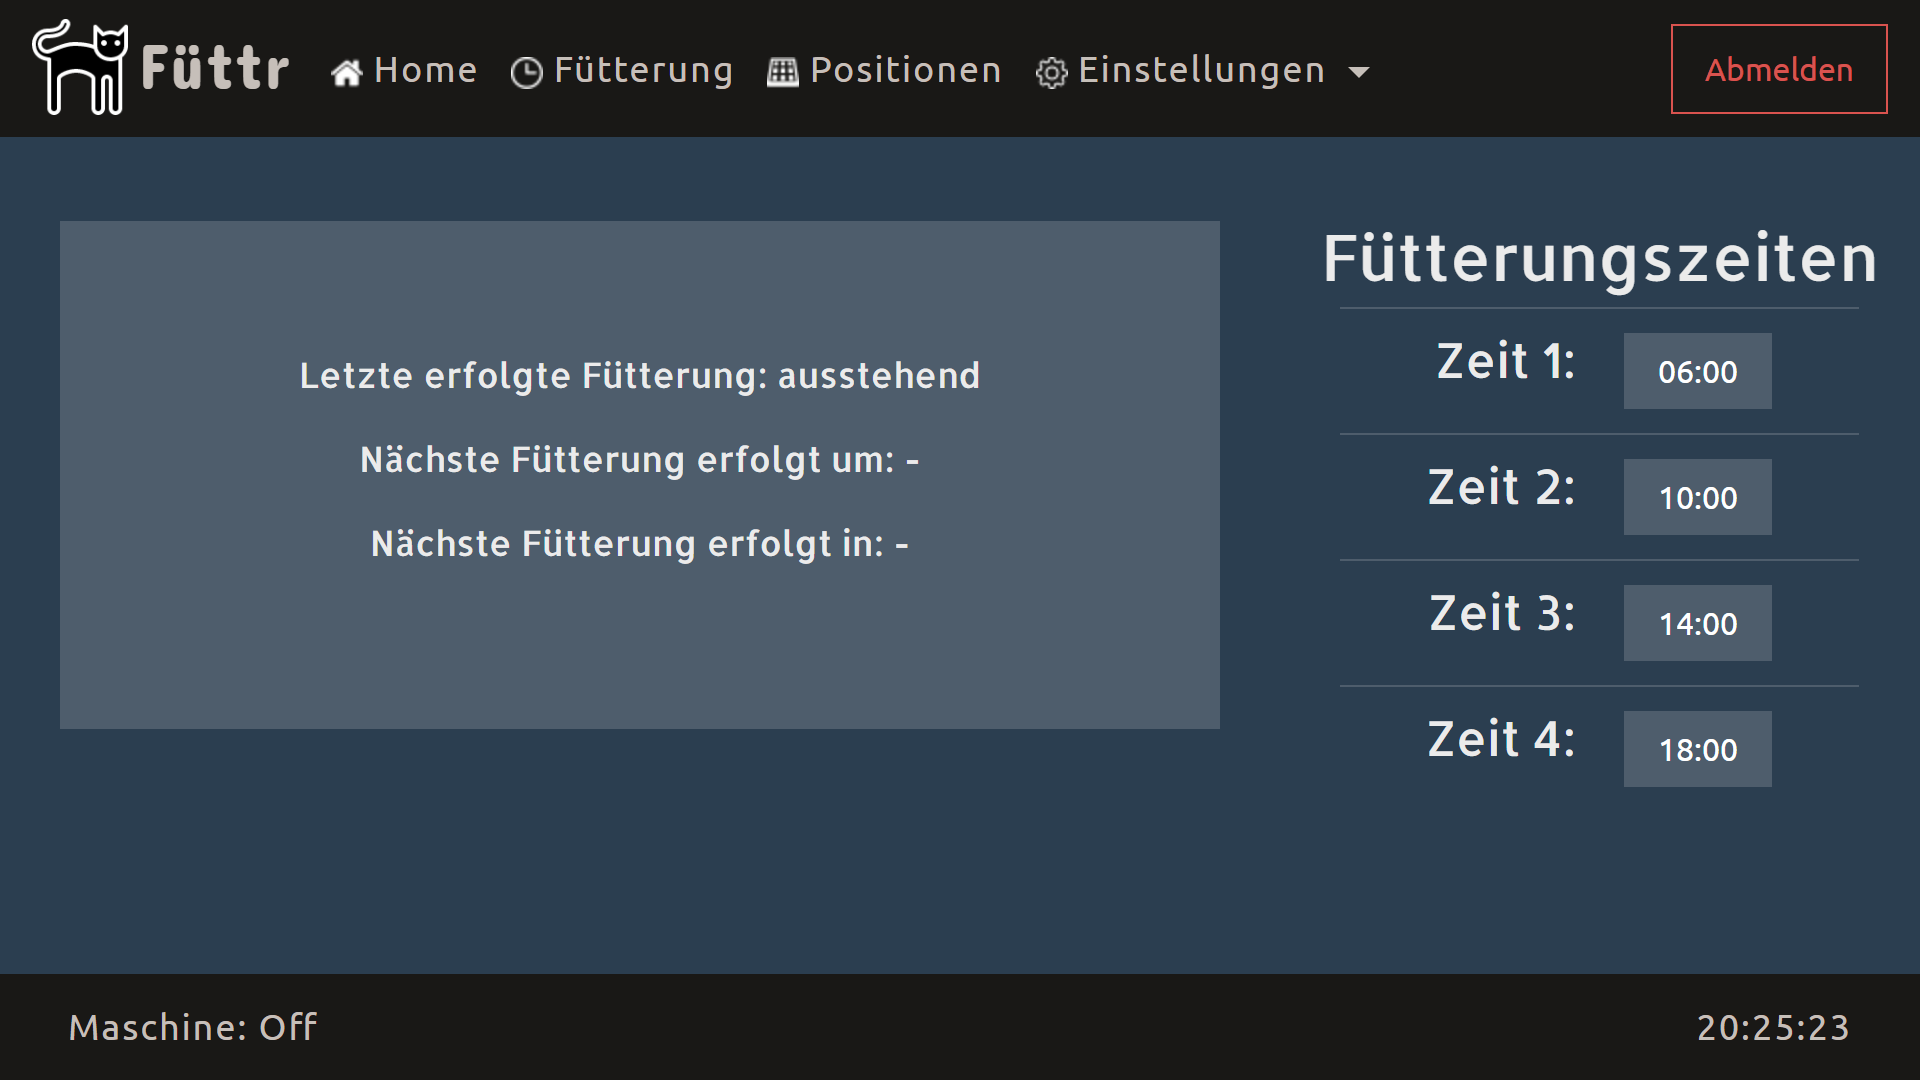
\includegraphics[width=0.65\textwidth]{Bilder/Greistorfer/Home}
  \end{center}
  \caption{Startseite}
  \label{Startseite}
  \vspace{-10pt}
\end{wrapfigure}

Auf der Startseite sind alle wichtigen Informationen übersichtlich dargestellt. Auf der linken Seite werden die Uhrzeit der letzten erfolgreichen Fütterung, die Zeit der nächsten Fütterung und die Zeit bis zur nächsten Fütterung dargestellt. Darunter werden Fehler und Warnungen, falls welche auftreten sollten, angezeigt. Da unbekannt ist, wie viele Fehler und Warnungen auftreten, werden diese in einem *ngFor aufgelistet. Auf der rechten Seite sind die aktiven Fütterungszeiten aufgelistet. \newpage

\begin{wrapfigure}{r}{0.7\textwidth}
\vspace{-10pt}
  \begin{center}
    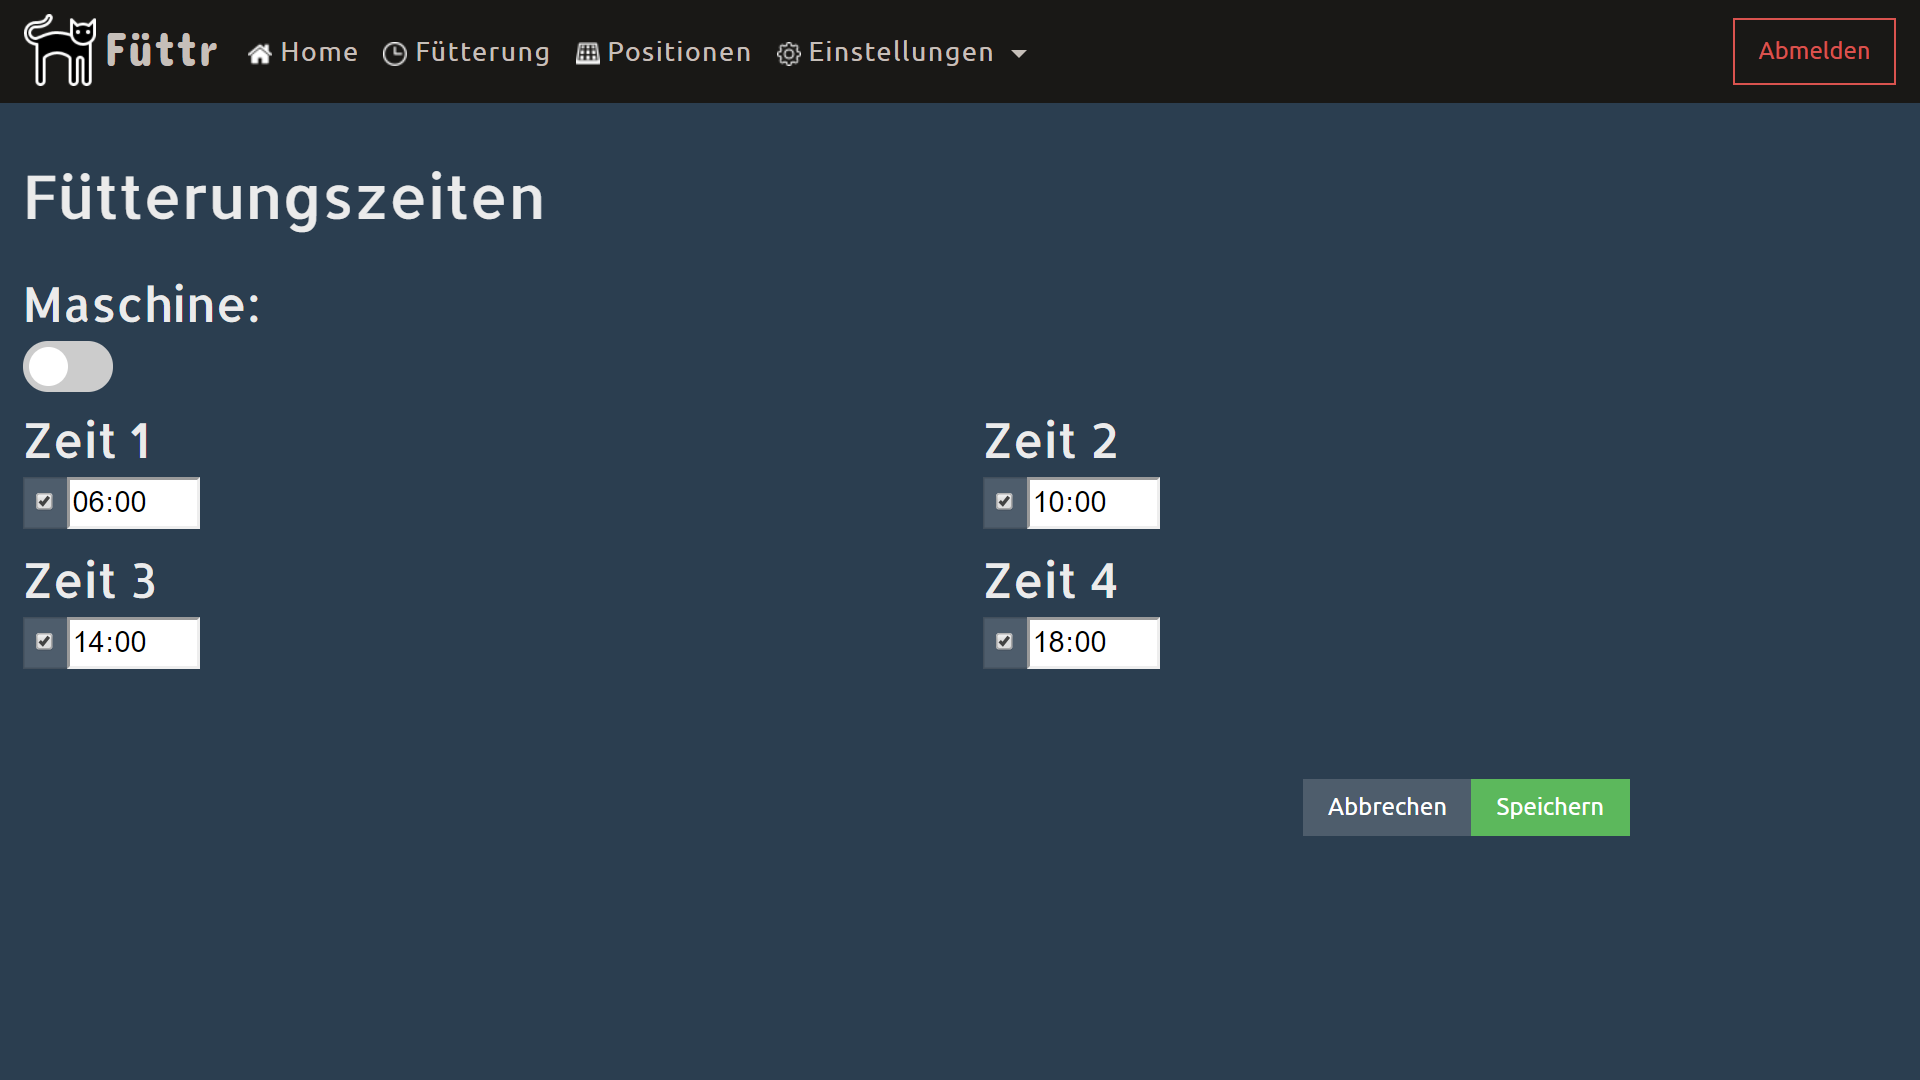
\includegraphics[width=0.65\textwidth]{Bilder/Greistorfer/Fuetterungszeiten}
  \end{center}
  \caption{Fütterungszeiten}
  \label{Fütterungszeiten}
  \vspace{-10pt}
\end{wrapfigure}

Auf der Fütterungszeiten-Seite kann der Benutzer die Katzenfütterungsanlage ein und ausschalten. Dies wurde mit einer Checkbox realisiert, die durch Styles wie ein Schalter gestaltet wurde. Darunter können die Fütterungszeiten geändert und deaktiviert werden. Siehe Abbildung \ref{Fütterungszeiten}. Der Button 'Speichern' wird deaktiviert, sobald eine Zeit ungültig eingegeben wurde oder wenn die Zeiten nicht in aufsteigender Reihenfolge sortiert sind. \\

\begin{wrapfigure}{r}{0.7\textwidth}
\vspace{-10pt}
  \begin{center}
    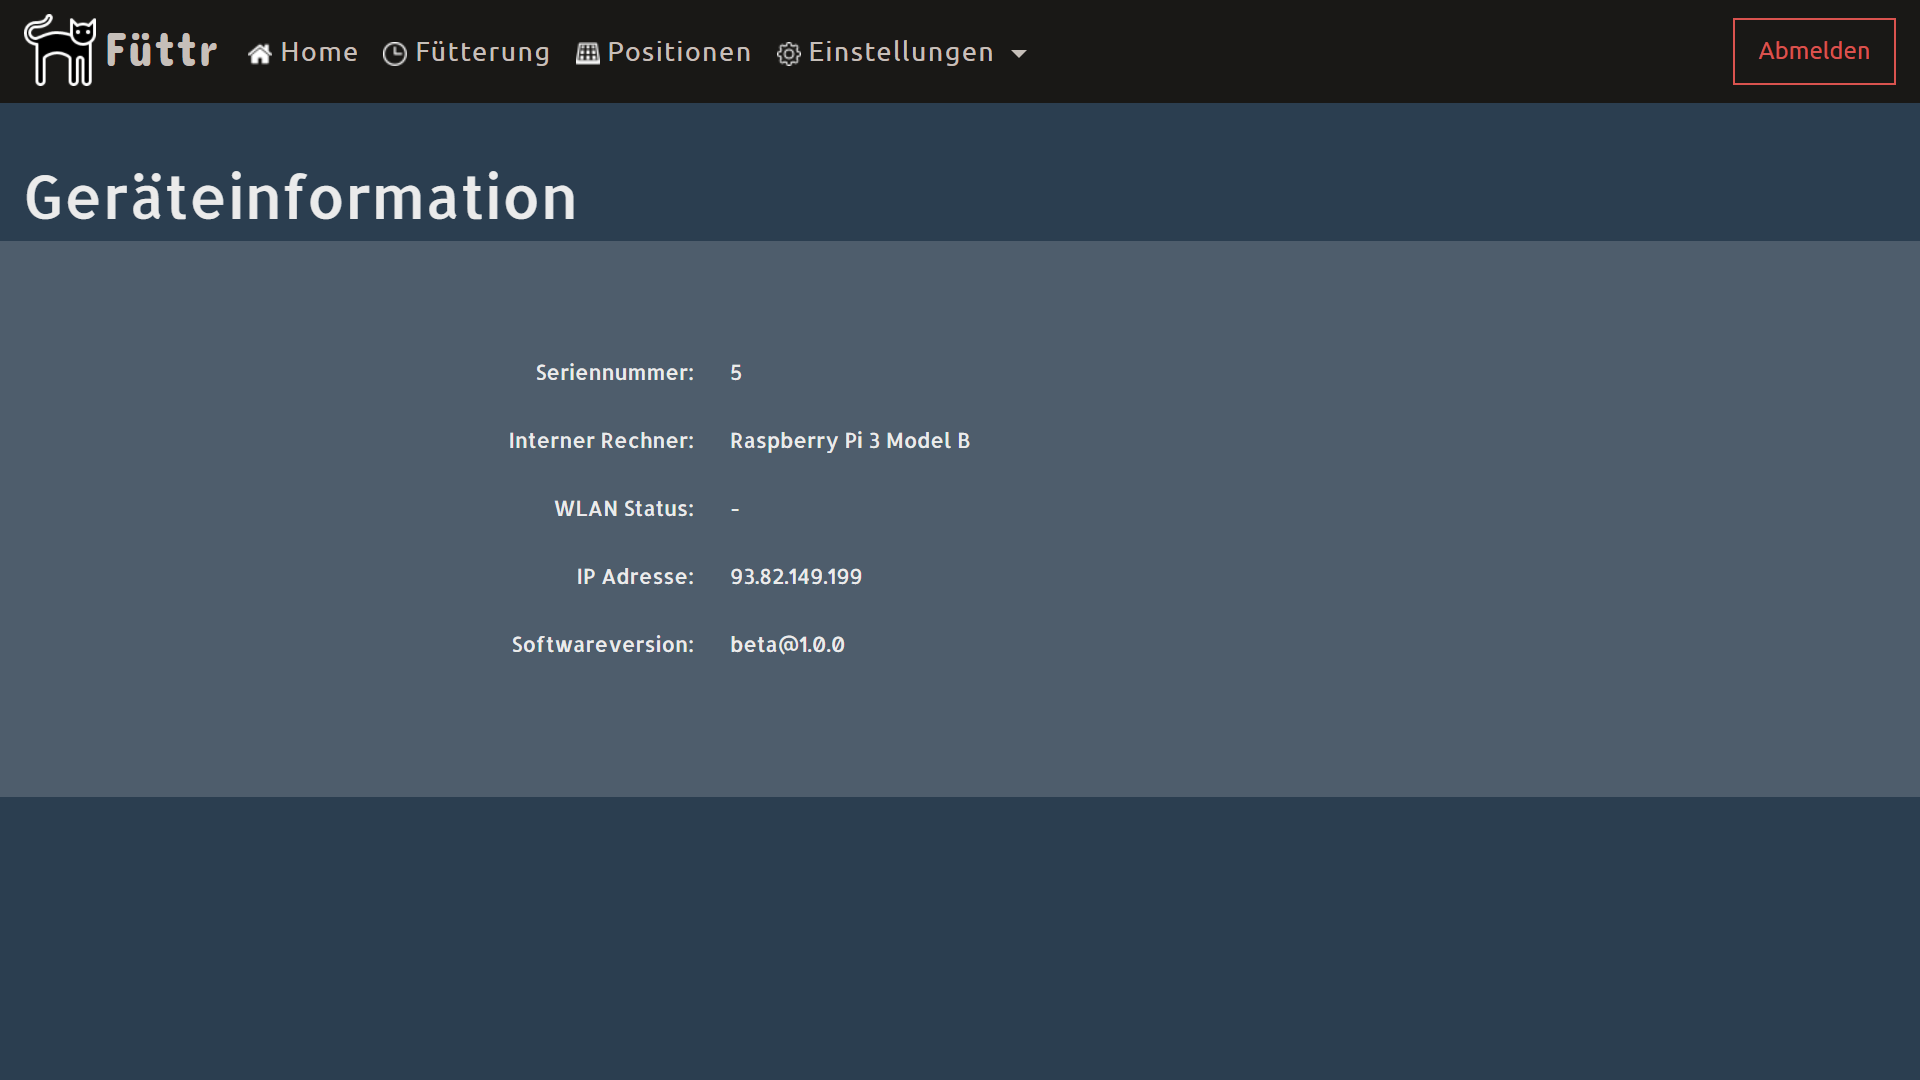
\includegraphics[width=0.65\textwidth]{Bilder/Greistorfer/Gerateinformation}
  \end{center}
  \caption{Geräteinformationen}
  \label{Geräteinformationen}
  \vspace{-60pt}
\end{wrapfigure}

Auf der Geräteinformations-Seite werden die wichtigsten Daten über das Gerät angezeigt. diese Daten sind:
\begin{itemize}
\item[•]Seriennummer
\item[•]Interner Rechner
\item[•]WLAN Status
\item[•]IP Adresse
\item[•]Softwareversion
\end{itemize}
Die IP-Adresse ist die aktuelle \textbf{externe} IP-Adresse. \newpage

\begin{wrapfigure}{r}{0.7\textwidth}
\vspace{-10pt}
  \begin{center}
    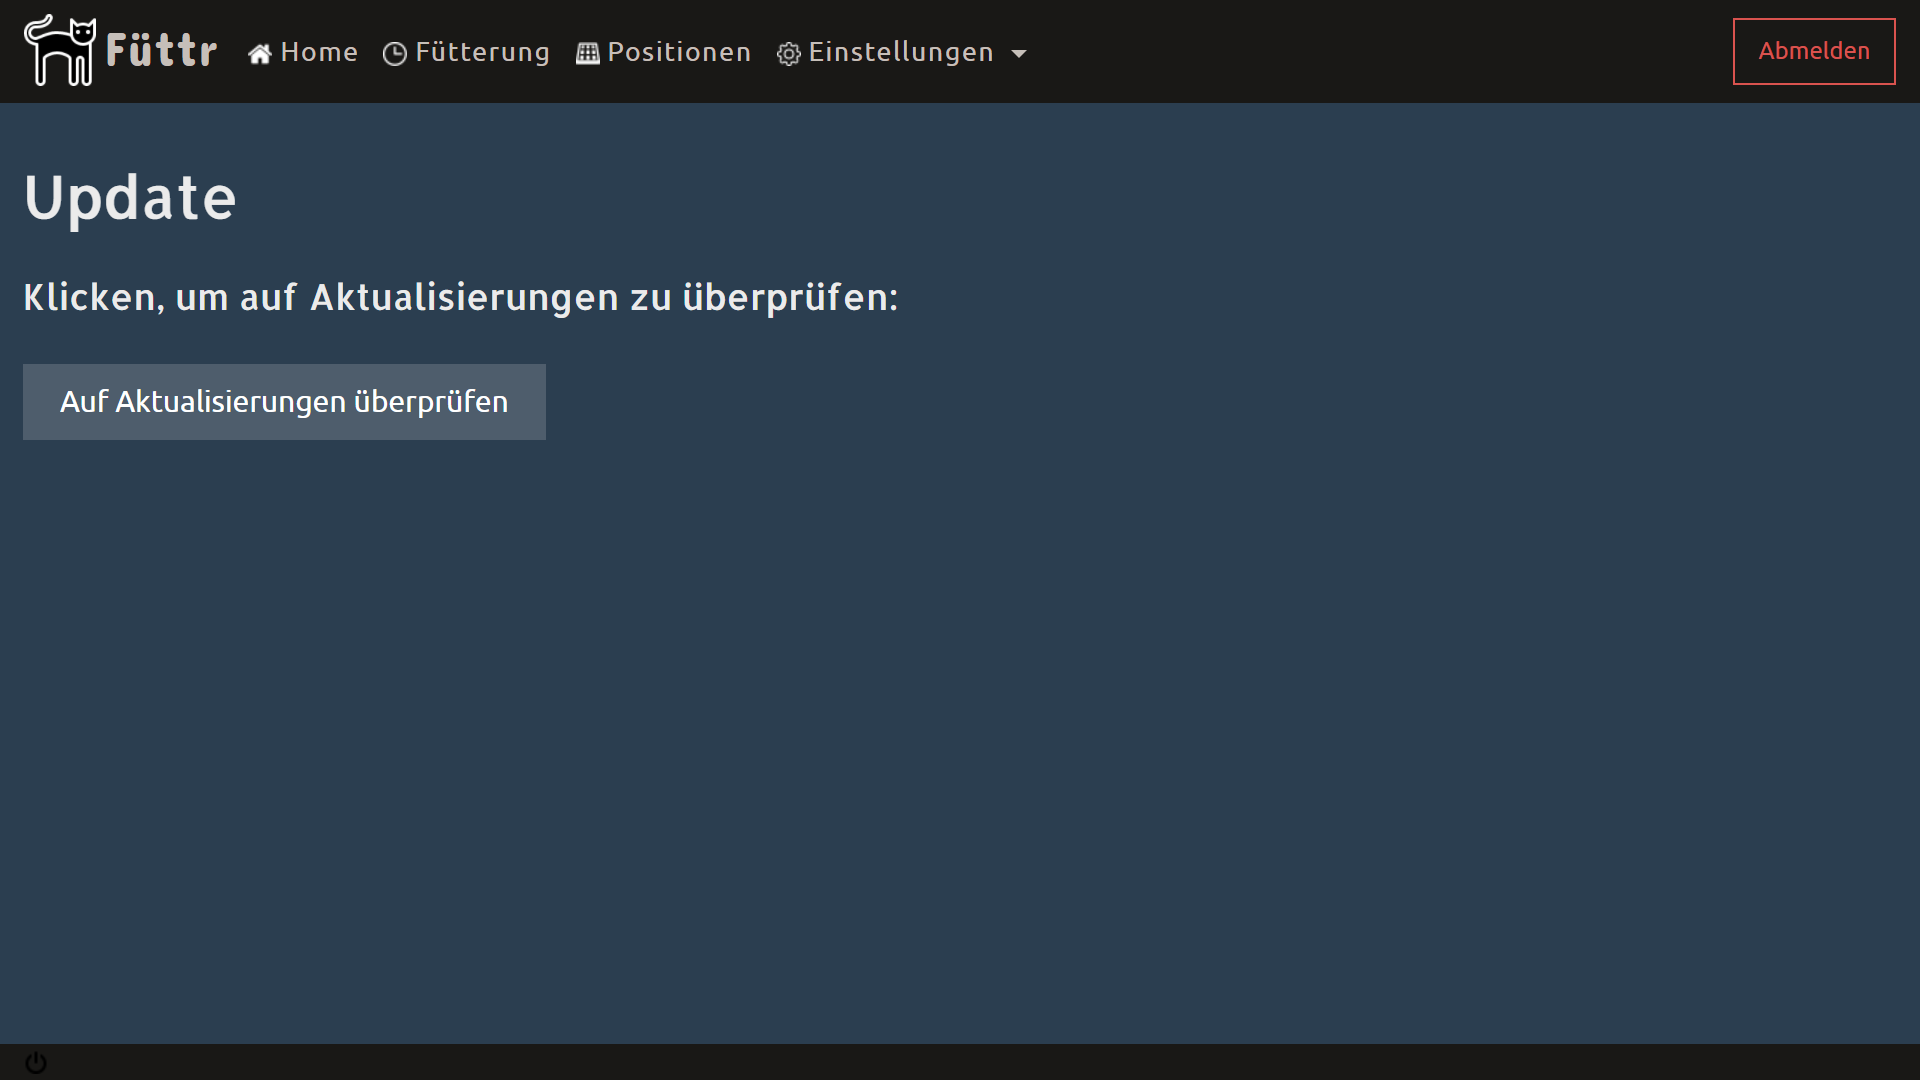
\includegraphics[width=0.65\textwidth]{Bilder/Greistorfer/Update}
  \end{center}
  \caption{Update}
  \label{Update}
  \vspace{-10pt}
\end{wrapfigure}

Auf der Update-Seite kann der Benutzer nach Updates suchen, Updates starten oder die Maschine herunterfahren. Wenn der Benutzer auf den Herunterfahren-Button klickt, der sich auf der linken Seite ganz unten befindet, wird er gewarnt, dass die Maschine nur mehr über das Aus- und wieder Einstecken des Netzteils startbar ist.\\

\subsubsection{Design}
\label{sec:ums-client-design}
Für das Design der Website wurde Bootstrap ausgewählt, da es bereits viele Positionierungsmöglichkeiten bietet und ohne viel Aufwand im Client verwendet werden kann. Bootstrap ist außerdem für Mobilgeräte und alle Bildschirmgrößen optimiert. Es bietet die Möglichkeit für Dropdownmenüs, Menüleisten und Popups. Diese Funktionen werden bei Bootstrap im Normalfall über JQuery\footnote{Mehr zu JQuery unter \url{https://jquery.com/}} gesteuert, aber da JQuery eine weitere externe JavaScript Bibliothek ist, wurde stattdessen das JavaScript Modul \textit{ng-bootstrap} verwendet. Dieses ist eine Erweiterung für Angular, mit dem sich die Bootstrap Komponenten steuern lassen. Damit dies funktioniert, muss \textit{ng-bootstrap} im \textit{Module} unserer Applikation eingebunden werden.

\begin{lstlisting}[caption=app.module (Auszug) Importieren von ng-bootstrap,label=import-ng-bootstrap,style=TS]
...
import { NgbModule, NgbDropdown } from '@ng-bootstrap/ng-bootstrap';
...
imports: [NgbModule.forRoot(), ...]
...
\end{lstlisting}

Da Bootstrap ohne etwas zu verändern etwas langweilig aussieht, entschied ich mich für das \textit{Superhero} Thema von der Seite \url{https://bootswatch.com/superhero/}. Da mir die orange Farbe nicht gefiel, änderte ich sie auf einen dunkleren Grauton, den ich aus einem Bild einer süßen Babykatze genommen habe. Bootstrap hat außerdem eine Standartschriftart, die ich geändert habe. Alle Schriftarten sind von der Seite \url{https://fonts.google.com/} genommen worden, da diese in Google's \ac{CDN} sind und somit ziemlich sicher die meiste Zeit verfügbar sind. Gewählt wurden die Schriftarten Ubuntu für alle Knöpfe und die Navigationsleiste, Allerta für alle Texte und Concert One für das Logo. Damit die Schrift auf allen Geräten gut lesbar ist und nicht zu groß wird, mussten die Schriftgrößen der Bildschirmbreite entsprechend angepasst werden.

\begin{lstlisting}[caption=Schriftgrößen entsprechend der Bildschirmbreite,label=css-font-sizes,style=css]
@media only screen and (max-width: 576px) {
  body {
    font-size: 0.5rem !important;
  }
  .bigger-h1 {
    font-size: 1.4rem !important;
  }
}
@media only screen and (max-width: 768px) {
  body {
    font-size: 0.7rem !important;
  }
  .bigger-h1 {
    font-size: 1.6rem !important;
  }
}
@media only screen and (max-width: 992px) {
  body {
    font-size: 0.9rem !important;
  }
  .bigger-h1 {
    font-size: 1.8rem !important;
  }
}
@media only screen and (max-width: 1200px) {
  body {
    font-size: 1.1rem !important;
  }
  .bigger-h1 {
    font-size: 2rem !important;
  }
}
\end{lstlisting}

Durch \inlinecode{css}{@media only screen and (max-width: ZAHLpx)} wird die Bildschirmbreite bestimmt und alle Styles innerhalb der Klammern werden nur dann angewandt, wenn der Ausdruck in der Klammer zutrifft. In der Klammer wird die Schriftgröße des \inlinecode{css}{body} Elements und allen Elementen der Klasse \inlinecode{css}{.bigger-h1} angepasst.

\paragraph*{Login}\mbox{}\\
Auf der Login Seite befindet sich rechts oben ein Dropdownmenü, in dem die Sprache geändert werden kann. Dies ist gelöst durch ein \inlinecode{HTML}{*ngFor}. Wenn das Menü geschlossen ist, wird dort die Flagge der aktuellen Sprache angezeigt, Österreich bei Deutsch und Großbritannien bei Englisch. Wenn man auf das Menü klickt, klappen alle Sprachen herunter, die zur Auswahl stehen und der Benutzer kann auf eine klicken. Die verschiedenen Auswahlmöglichkeiten sind Links, die den Benutzer auf den jeweiligen Sprachcode umleiten und die Seite somit in der gewünschten Sprache anzeigen. In der Mitte der Seite befindet sich ein Bootstrap Jumbotron. Ein Jumbotron ist dafür gedacht, auf etwas Aufmerksamkeit zu ziehen. Damit verändert sich die Hintergrundfarbe und es entsteht eine klare Abhebung. Innerhalb des Jumbotrons ist ein \ac{HTML} Formular, in das der Benutzername und das Passwort vom Benutzer hineingeschrieben werden. Beim Klick auf den Knopf \textit{Anmelden} werden diese Daten dem Server übermittelt. Sollte das Anmelden geglückt sein, so wird automatisch die Startseite angezeigt. Auf allen weiteren Seiten ist rechts oben ein Knopf, mit dem sich der Benutzer abmelden kann.

\paragraph*{Startseite}\mbox{}\\
Auf der linken Seite befindet sich ein Jumbotron, in dem die letzte Fütterungszeit, die nächste Fütterungszeit und die Zeit bis zur nächsten Fütterung angezeigt werden. Auf der rechten Seite werden die aktiven Fütterungszeiten angezeigt. Sollte eine Zeit deaktiviert werden, so wird sie auch nicht in dieser Liste angezeigt. Der Jumbotron und die Liste sind mithilfe von Bootstrap in einem Verhältnis von 2:1 nebeneinander angeordnet. Sollte die Bildschirmbreite zu klein werden, entweder, weil die Seite auf einem Mobilgerät angezeigt wird, oder weil der Benutzer das Browserfenster klein darstellt, so werden die beiden Elemente untereinander dargestellt. Unterhalb des Jumbotrons werden auftretende Fehler und Warnungen angezeigt. Dies ist wiederum mit zwei \inlinecode{HTML}{*ngFor} gelöst. Die Fehler und Warnungen sind Bootstrap Alerts. Sie sind dafür gedacht, dem Benutzer auf etwas aufmerksam zu machen. Sie können durch ein x auf der rechten Seite geschlossen werden. Am unteren Bildschirmrand ist eine Leiste, die die gleiche Farbe wie die Navigationsleiste hat. Auf ihr wird links angezeigt, ob die Maschine ein- oder ausgeschalten ist.

\paragraph*{Fütterungszeiten}\mbox{}\\
Unter der Überschrift befindet sich ein Schalter, der es dem Benutzer ermöglicht, die MAschine ei- und auszuschalten. Dieser Schalter ist eine normale \ac{HTML} Checkbox, die durch \ac{CSS} Styling wie ein Schalter designet wurde.

\begin{lstlisting}[caption=HTML Schalter,label=html-schalter,style=HTML]
<label class="switch">
  <input type="checkbox" [(ngModel)]="machine_state">
  <span class="slider"></span>
</label>
\end{lstlisting}

\begin{lstlisting}[caption=CSS Schalter,label=css-schalter,style=css]
.switch {
  position: relative;
  display: inline-block;
  width: 60px;
  height: 34px;
}

.switch input {
  display: none;
}

.slider {
  border-radius: 34px;
  position: absolute;
  cursor: pointer;
  top: 0;
  left: 0;
  right: 0;
  bottom: 0;
  background-color: #ccc;
  -webkit-transition: 0.4s;
  transition: 0.4s;
}

.slider :before {
  border-radius: 50%;
  position: absolute;
  content: '';
  height: 26px;
  width: 26px;
  left: 4px;
  bottom: 4px;
  background-color: white;
  -webkit-transition: 0.4s;
  transition: 0.4s;
}

input :checked + .slider {
  background-color: #2196f3;
}

input :focus + .slider {
  box-shadow: 0 0 1px #2196f3;
}

input :checked + .slider :before {
  -webkit-transform: translateX(26px);
  -ms-transform: translateX(26px);
  transform: translateX(26px);
}
\end{lstlisting}

Mit dem \inlinecode{css}{:before} Selector wird ein Element vor dem tatsächlichen Element eingefügt. Dies wird gemacht, da das \textit{input} Element nicht so dargestellt werden kann, wie wir es gerne möchten. Mit \inlinecode{css}{display: none;} blenden wir das \textit{input} Element aus. Mit \inlinecode{css}{transform:}, \inlinecode{css}{-webkit-transform:} und \inlinecode{css}{-ms-transform:} wird der Schalter animiert und es wird sichergestellt, dass alle herkömmlichen Browser es unterstützen. Darunter kann der Benutzer die Fütterungszeiten einstellen. Die \textit{input} Elemente sind durch Bootstrap in zwei Spalten im Verhältnis 1:1 angeordnet. Darunter befinden sich zwei Knöpfe, mit denen man die Eingabe der Zeiten abbrechen und bestätigen kann. Bei erfolgreicher Speicherung wird neben dem Speichern ein Knopf eingeblendet, auf dem \textit{Gespeichert} steht. Dies wird durch Angular Animationen ermöglicht, siehe \autoref{par:funk-fuettr}. Sollte das Speichern fehlschlagen, sei es durch Verbindungsprobleme oder einem falschen bzw. abgelaufenen Tokens, so wird unter dem Speichern Knopf über die ganze Seite ein Alert angezeigt, der dem Benutzer mitteilt, dass das Speichern fehlgeschlagen ist. Alle Eingegebenen Daten werden laufend überprüft, siehe \autoref{par:funk-fuettr}.

\paragraph*{Positionen}\mbox{}\\
Auf dieser Seite befinden sich vier Elemente, die mithilfe von Bootstrap in vier gleich großen Spalten angeordnet sind. Wenn die Bildschirmbreite zu klein wird, so werden sie untereinander angezeigt.

\paragraph*{Geräteinformationen}\mbox{}\\
In der Mitte der Seite befindet sich ein Jumbotron, der die ganze Seitenbreite umfasst. In ihm ist eine Tabelle, die mit der Bootstrap Klasse \inlinecode{css}{.table-hover} gestyled wurde. Diese Klasse bewirkt, dass die Zeile, über die der Mauszeiger sich gerade befindet, hervorgehoben wird. Dadurch kann der Benutzer leichter erkennen, in welcher Zeile er gerade liest.

\paragraph*{Aktualisierungen}\mbox{}\\
Auf dieser Seite befindet sich nur ein Knopf in der Mitte, der ein Popup, ein sogenanntes Modal, anzeigt. Dies ist durch \textit{ng-bootstrap} gelöst. Bei Aufruf der Seite wird überprüft, ob eine Softwareaktualisierung verfügbar ist. Im Modal wird dann angezeigt, ob eine Aktualisierung verfügbar ist und wie lange es gedauert hat, bis die Überprüfung abgeschlossen war. Sollte eine Aktualisierung verfügbar sein, so wird ein Knopf angezeigt, über den der Benutzer den Aktualisierungsvorgang starten kann. Wird der Aktualisierungsvorgang gestartet, so wird der Knopf deaktiviert, sodass er nicht mehr anklickbar ist. Ein Ladebalken zeigt dem Benutzer, dass der Vorgang unbestimmte Zeit dauert. In dem Ladebalken steht ein Text, der dem Benutzer mitteilt, in welchem Stadium das Raspberry sich befindet, siehe \autoref{par:funk-upd}.

\subsubsection{Funktion}
\label{sec:ums-client-funktion}

\paragraph*{Struktur} \mbox {}\\
Der Haupt-\textit{Component}, der geladen wird, wenn die Seite aufgerufen wird, ist \textit{app.component}. In seinem Template ist die Navigationsleiste, die sich alle Seiten teilen. Alle weiteren Seiten werden im \inlinecode{html}{<router-outlet></router-outlet>} angezeigt. Das ist ein \ac{HTML}-Tag der von Angulars Router zur Verfügung gestellt wird. Ein Router ist ein Service, welches das Navigieren der Seite ermöglicht. Damit das funktioniert, muss dem Router mitgeteilt werden, wie die Seite aufgebaut ist. Dies geschieht im \textit{router.module}:

\begin{lstlisting}[caption=Routes Definition,style=TS]
const routes: Routes = [
  { path: 'home', component: HomeComponent, 
  		data: { title: 'Füttr' }, canActivate: [AuthGuard]},
  { path: '', pathMatch: 'full', redirectTo: 'login'},
  { path: 'login', component: LoginComponent,
  		data: { title: 'Füttr - Login' }},
  { path: 'position', component: PositionComponent, 
  		data: { title: 'Füttr - Positions' }, canActivate: [AuthGuard]},
  { path: 'feed', component: FeedComponent, 
  		data: { title: 'Füttr - Feeding-Cycle' }, canActivate: [AuthGuard},
  { path: 'info', component: InfoComponent, 
  		data: { title: 'Füttr - Info' }, canActivate: [AuthGuard]},
  { path: 'update', component: UpdateComponent, 
  		data: { title: 'Füttr - Update' }, canActivate: [AuthGuard]},
  { path: '**', component: Error404Component, 
  		data: { title: 'Füttr - 404 (not found)'}}
];
\end{lstlisting}

Jede Route bekommt ein data Objekt übergeben, das bei Aufruf der \textit{Component} dem @Input Decorator injiziert wird. Der jeweilige \textit{Component} ändert damit den Titel der Seite. Alle Routes, außer \textit{login} und \textit{404} sind von einem AuthGuard geschützt, das bedeutet, nur authorisierte Benutzer können diese Routes aufrufen. Der Request auf \textit{root} \inlinecode{TS}{path: ''} wird umgeleitet auf \textit{login}. Für jeden Request, dessen Route nicht definiert ist, wird der 404 Component geladen: \inlinecode{TS}{path: '**'}. Um auf eine andere Seite innerhalb der Applikation zu gelangen, gibt es zwei Möglichkeiten. Einmal über ein \ac{HTML} Element, auf das der Benutzer klickt mittels \ac{HTML} Attribut \inlinecode{HTML}{routerLink} oder auf der TypeScript Seite.

\begin{lstlisting}[caption=Weiterleitung mittels \ac{HTML} Attributes,label=html-redirect,style=HTML]
<a class="nav-link" routerLink="/feed" i18n>...</a>
\end{lstlisting}

\begin{lstlisting}[caption=Weiterleiten mittels TypeScript,label=ts-redirect,style=TS]
this.router.navigateByUrl('/home');
\end{lstlisting}

\paragraph*{\ac{HTTP} Service}\mbox{}\\
Da alle \textit{Components} Daten vom Server holen und manche auch Daten zum Server schicken, war es die logische Schlussfolgerung, ein Service zu erstellen, das jede Art von \ac{HTTP} Anfrage verarbeiten kann. Dieses Service ist \textit{http.service}. Alle Anfragen, egal ob \textit{GET} oder \textit{PUT} werden von diesem Service getätigt. Das Service importiert Angular's \textit{HttpClient}, mit dem es sehr einfach ist, Anfragen zu erstellen und die Antworten zu verarbeiten. Die Antworten vom Server sind vom Typ \textit{application/json}, das bedeutet, sie sind \ac{JSON}-Dateien, die der \textit{HttpClient} dann in Objekte umwandelt. Diese Objekte werden dem \textit{Component} übergeben, sobald die Anfrage abgeschlossen wurde.

\paragraph*{Fütterungszeiten}\mbox{}\\
\label{par:funk-fuettr}
Die Eingabe wurde realisiert durch \ac{HTML} input Elemente vom Typ \textit{time}. Da \textit{time} browserabhängig ist und ältere Browser es als \textit{text} interpretieren könnten, und die Application auf allen Browsern funktionieren soll, werden alle Eingabefelder auf Richtigkeit überprüft. Außerdem sollen alle Zeiten in aufsteigender Reihenfolge eingegeben werden. Der \textit{time} Typ ist eigentlich nur ein string, das bedeutet, um die Reihenfolge zu überprüfen, müssen diese zuerst in Zahlen umgewandelt werden. Das geht mit der Funktion \inlinecode{TS}{parseInt()}. Ein string von einem \textit{time} input sieht meistens so aus: \inlinecode{TS}{'12:34'} Wenn die Zeit leer ist, sieht er so aus: \inlinecode{TS}{'--:--'} Auf diese beiden Arten muss unser Parser vorbereitet sein. Der Parser wandelt den string in Minuten um, danach werden sie verglichen. Sollte eine Zeit ungültig sein oder sollte eine Zeit außer Reihenfolge sein, so wird der Speicher-Button deaktiviert. Überprüft wird, sobald der User etwas ändert. Dies geschieht durch den DoCheck() Lifecycle Hook (siehe \ref{sec:ang-components}). Über den Fütterungszeiten kann man außerdem die Maschine ein und ausschalten.

\begin{lstlisting}[caption=Zeiten Parser,style=TS,label=zeiten_parser,captionpos=t]
toMinutes(time: string): number {
  let timeHours: number;
  let timeMinutes: number;
  if (time[0] === '-' && time[1] === '-' 
      && time[3] === '-' && time[4] === '-') {
    return null;
  }
  timeHours = parseInt(time[0], 10) * 10;
  timeHours = timeHours + parseInt(time[1], 10);
  timeMinutes = parseInt(time[3], 10) * 10;
  timeMinutes = timeMinutes + parseInt(time[4], 10);
  return timeHours * 60 + timeMinutes;
}
\end{lstlisting}

Neben dem Speichern Knopf wird bei erfolgreicher Speicherung ein weiterer Knopf animiert. Dies geschieht durch Angular Animationen.

\begin{lstlisting}[caption=Animieren des Knopfs,label=button-animation,style=TS]
animations: [
  trigger('SaveAnimation', [
    state('false', style({ opacity: '0.0' })),
    state('true', style({ opacity: '1.0' })),
    transition('* => *', animate('300ms'))
  ]),
  trigger('FailAnimation', [
    state('false', style({ opacity: '0.0' })),
    state('true', style({ opacity: '1.0' })),
    transition('* => *', animate('300ms'))
  ])
]
\end{lstlisting}

Bei dem zu animierenden Element wird \inlinecode{HTML}{[@NameDerAnimation]="auslöserVariable"} in die Attribute geschrieben. Ändert sich diese Variable, so wird die Animation gestartet. Animiert werden kann alles, dass durch Styles bestimmt werden kann.

\paragraph*{Updates}\mbox{}\\
\label{par:funk-upd}
Auf der Updates Seite kann der Benutzer nach neuen Updates suchen und das Gerät updaten. Realisiert wurde dies durch eine Anfrage an Github, wo eine Datei namens \textit{version.json} liegt. Diese wird verglichen mit der Datei, die auf dem System liegt. Dieser Vergleich geschieht bereits im OnInit() Lifecycle Hook (siehe \ref{sec:ang-components}). Der User kann nochmal nach Updates suchen, wenn er dies möchte. Sollte ein Update verfügbar sein, so wird der Button aktiv und der Benutzer kann sich dazu entscheiden, dass Gerät upzudaten. Wird aktualisiert, so wird eine Anfrage an den Server gesendet siehe \ref{sec:ums-server-funktion}. Der Client beginnt, dauerhaft Anfragen zu senden, bis eine fehlschlägt. Eine Nachricht teilt dem Benutzer mit, dass das System aktualisiert. Dann werden so lange Anfragen gesendet, bis wieder eine Antwort ankommt. Dann wird die Seite automatisch neu geladen. Der Updatevorgang ist damit abgeschlossen.

\paragraph*{Login}\mbox{}\\
Das Login funktioniert auf der Basis des Angular Auth Guards. Dieser schützt gewisse Routes gegen unbefugte Benutzer. Im Login bekommen wir, bei erfolgreicher Authentifikation einen \ac{JWT} vom Server, den wir in einer Variable speichern und dann im \inlinecode{bash}{Authorization} Header bei Bedarf mitschicken. Dies geschieht durch einen sogenannten \textit{Interceptor}, der den \ac{HTTP} Request nimmt und ihn klont, da \ac{HTTP} Requests in Angular nicht veränderbar sind, und dann zusätzlich den \inlinecode{bash}{Authorization} Header hinzufügt.

\subsubsection{Internationalization}
\label{sec:ums-client-i18n}
Um die Webseite in mehreren Sprachen anzeigen zu können, muss sie in allen Sprachen extra übersetzt sein. Das würde bedeuten, für jede Sprache wird ein eigenes Angular Projekt benötigt. Das wäre sehr viel Speicherplatz und Rechenleistung. Glücklicherweise bietet Angular eine Möglichkeit, die App in mehrere Sprachen zu übersetzen, ohne die ganze App neu zu schreiben. Diese Möglichkeit nennt sich Internationalization oder kurz i18n. Angluar muss nur wissen, welche Teile wie übersetzt werden sollen. Dafür schreiben wir bei allen \ac{HTML} Elementen, deren Text wir übersetzen wollen i18n zu den Attributen. \inlinecode{Html}{<h4 i18n>Zeit 1:</h4>}. Mit dem Kommando \inlinecode{bash}{ng xi18n --output-path src/i18n} werden alle Texte in eine Datei namens \textit{messages.xlf} extrahiert. Diese Datei wird dann kopiert, für jede Sprache eine neue Datei. Jede Datei wird entsprechend des Sprachencodes umbenannt, für Deutsch wäre das \textit{messages.de.xlf}. In dieser Datei steht jeder Text in einem \inlinecode{bash}{<source>} Tag. Diese Texte werden übersetzt und unterhalb in einen \inlinecode{bash}{<target>} Tag geschrieben. Im Falle dieser Arbeit wurden die Texte alle in Deutsch und Englisch übersetzt. Zum Bauen des mehrsprachigen Projekts muss Angular mitgeteilt werden, welche Sprachen und welche Dateien es verwenden soll. Unter Linux geht das mit dem Kommando \inlinecode{bash}{for lang in en de; do ng build --output-path}\\\inlinecode{bash}{=dist/\$lang --aot --prod --bh \$lang/ --i18n-file=src/i18n/messages.\$lang.xlf}\\\inlinecode{bash}{--i18n-format=xlf --locale=\$lang; done}. Dieses Kommando baut unsere Applikation in den \textit{dist} Ordner, jede Sprache bekommt dabei ihren eigenen Unterordner, der dem Sprachencode entspricht.

\subsubsection{Kommunikation mit dem Server}
\label{sec:ums-client-kommunikation}
Der Client benötigt viele Daten vom Server und sendet einige an den Server. Das Übertragungsprotokoll, Tabelle \ref{webserver-client-uebertragung}, gibt klare Auskunft über alle mögliche Anfragen und Antworten.
\begin{landscape}
\begin{table}[]
\begin{tabular}{@{}llll@{}}
\toprule
\multicolumn{1}{|l|}{\textbf{\ac{HTTP} Request Typ}} & \multicolumn{1}{l|}{\textbf{\ac{URI}}} & \multicolumn{1}{l|}{\textbf{Server Response}} & \multicolumn{1}{l|}{\textbf{Beispiel}}                                                                                                          \\ \midrule
\multicolumn{1}{|l|}{GET}  & \multicolumn{1}{l|}{/api/ip}                             & \multicolumn{1}{l|}{IP}                  & \multicolumn{1}{l|}{\footnotesize{\ttfamily{\{''ip":"62.116.40.166"\}}}}                                                                                                                                                                                                                       \\ \midrule
\multicolumn{1}{|l|}{GET}  & \multicolumn{1}{l|}{/api/version}                        & \multicolumn{1}{l|}{Version}             & \multicolumn{1}{l|}{\footnotesize{\ttfamily{\{"version": "beta@1.0.0"\}}}}                                                                                                                                                                                                                     \\ \midrule
\multicolumn{1}{|l|}{GET}  & \multicolumn{1}{l|}{/api/getUpdate}                      & \multicolumn{1}{l|}{200 OK}              & \multicolumn{1}{l|}{}                                                                                                                                                                                                                                                \\ \midrule
\multicolumn{1}{|l|}{GET}  & \multicolumn{1}{l|}{/api/shutdown}                       & \multicolumn{1}{l|}{200 OK}              & \multicolumn{1}{l|}{}                                                                                                                                                                                                                                                \\ \midrule
\multicolumn{1}{|l|}{GET}  & \multicolumn{1}{l|}{/api/callMeMaybe/times}            & \multicolumn{1}{l|}{Zeiten}              & \multicolumn{1}{l|}{\footnotesize{\ttfamily{\begin{tabular}[c]{@{}l@{}}\{"time1":"12:20","time1\_active":true,\\"time2":"13:20","time2\_active":true,\\"time3":"14:20","time3\_active":true,\\"time4":"15:20","time4\_active":true\}\end{tabular}}}}                                           \\ \midrule
\multicolumn{1}{|l|}{GET}  & \multicolumn{1}{l|}{/api/callMeMaybe/status}           & \multicolumn{1}{l|}{Status}              & \multicolumn{1}{l|}{\footnotesize{\ttfamily{\begin{tabular}[c]{@{}l@{}}\{"nextFeeding":"-","lastFeeding":\\''ausstehend","nextFeedingIn":''-'',\\"machineState":false\}\end{tabular}}}}                                                                                                            \\ \midrule
\multicolumn{1}{|l|}{GET}  & \multicolumn{1}{l|}{/api/callMeMaybe/info}             & \multicolumn{1}{l|}{Info}                & \multicolumn{1}{l|}{\footnotesize{\ttfamily{\begin{tabular}[c]{@{}l@{}}\{''serialnumber":"17",''internal":"Raspberry\\Pi 3 Model B", "wlanState":"not connected"\}\end{tabular}}}}                                                                                                            \\ \midrule
\multicolumn{1}{|l|}{GET}  & \multicolumn{1}{l|}{/api/callMeMaybe/positions}        & \multicolumn{1}{l|}{Positionen}          & \multicolumn{1}{l|}{\footnotesize{\ttfamily{\begin{tabular}[c]{@{}l@{}}\{"motor1":''-'',"motor2":''-'',''sensor1":''-'',\\''sensor2":''-''\}\end{tabular}}}}                                                                                                                                                                                         \\ \midrule
\multicolumn{1}{|l|}{GET}  & \multicolumn{1}{l|}{/api/callMeMaybe/errors\_warnings} & \multicolumn{1}{l|}{Errors und Warnings} & \multicolumn{1}{l|}{\footnotesize{\ttfamily{\begin{tabular}[c]{@{}l@{}}\{''Errors":{[}\{"message":''Error","hidden":\\false\}{]},"Warnings":{[}\{"message":"Warning",\\"hidden":false\}{]}\}\end{tabular}}}} \\ \midrule
\multicolumn{1}{|l|}{POST} & \multicolumn{1}{l|}{/api/putMeHere/times}              & \multicolumn{1}{l|}{Zeiten}              & \multicolumn{1}{l|}{\footnotesize{\ttfamily{\begin{tabular}[c]{@{}l@{}}\{"time1":"12:20","time1\_active":true,\\"time2":"13:20","time2\_active":true,\\"time3":"14:20","time3\_active":true,\\"time4":"15:20","time4\_active":true\}\end{tabular}}}}                                           \\ \midrule
\multicolumn{1}{|l|}{POST} & \multicolumn{1}{l|}{/api/putMeHere/changeState}        & \multicolumn{1}{l|}{Status}              & \multicolumn{1}{l|}{\footnotesize{\ttfamily{\{''state":"true"\}}}}                                                                                                                                                                                                                             \\ \midrule
\multicolumn{1}{|l|}{POST} & \multicolumn{1}{l|}{/login}                              & \multicolumn{1}{l|}{\ac{JWT}}          & \multicolumn{1}{l|}{\footnotesize{\ttfamily{\{"token":"...",''isLoggedIn":true\}}}}                                                                                                                                                                                                             \\ \midrule
\multicolumn{1}{|l|}{POST} & \multicolumn{1}{l|}{/logout}                             & \multicolumn{1}{l|}{200 OK}              & \multicolumn{1}{l|}{}                                                                                                                                                                                                                                                \\ \bottomrule
\end{tabular}
\caption{Übertragungsprotokoll Webserver - Webclient}
\label{webserver-client-uebertragung}
\end{table}
\end{landscape}

\subsection{Server}
\label{sec:ums-server}

\subsubsection{Serverpfade}
\label{sec:ums-server-pfade}

\paragraph*{GET}\mbox{}\\
\begin{forest}
	[\textit{root}
		[api
			[version]
			[callMeMaybe
				[times]
				[status]
				[info]
				[positions]
				[errors\_warnings]			
			]
			[getUpdate]
			[shutdown]
			[ip]		
		]
		[de]
		[en]
	]
\end{forest}

\paragraph*{POST}\mbox{}\\
\begin{forest}
	[\textit{root}
		[api
			[putMeHere
				[times]
				[changeState]			
			]	
		]
		[login]
		[logout]	
	]
\end{forest}


\subsubsection{Funktion}
\label{sec:ums-server-funktion}
Da auf einem Port nur ein Programm auf Anfragen warten kann und sichergestellt sein soll, dass der Server nur einmal gestartet wird, wird der Server als Singleton ausgeführt. Das bedeutet, der Konstruktor der Klasse ist nicht öffentlich. Stattdessen gibt es einen Getter, der überprüft, ob ein Objekt der Klasse bereits existiert. Sollte ein Objekt bereits erstellt sein, so wird dieses zurückgegeben. Existiert noch kein Objekt, so wird eines erstellt und danach zurückgegeben. Der Server wir gestartet, indem dem Node.js Modul \textit{http} das Server Objekt übergeben wird: \inlinecode{TS}{const server = http.createServer(this._express).listen(port)}

\begin{lstlisting}[caption=Server Singleton,label=server_singleton,style=TS]
public static get Instance(): Server {
  if (Server._instance === undefined) {
    Server._instance = new Server();
  }
  return Server._instance;
}
\end{lstlisting}

Der Server wurde mit dem JavaScript Modul \textit{express} programmiert. Express ist aufgebaut mit sogenannten Middlewares. Diese werden bei Eintreffen einer Anfrage der Reihe nach durchgegangen, bis eine Middleware der Anfrage entspricht. Wenn z.B. die Anfrage \inlinecode{bash}{HTTP/1.1 GET /api/version} eintrifft, werden die Middlewares nach der Reihe durchgegangen. Jede Middleware mit \inlinecode{TS}{use}, solange kein Pfad mit angegeben wurde, wird ausgeführt, alle anderen werden übersprungen. Die nächste Middleware, die ausgeführt wird, ist \inlinecode{TS}{get('/api/version', ...)}. Wird in dieser Middleware \inlinecode{TS}{next()} aufgerufen, so werden alle weiteren Middlewares durchgegangen. Sollte \inlinecode{TS}{next()} nicht aufgerufen werden, so werden keine weiteren Middlewares durchgegangen.

\begin{lstlisting}[style=TS,caption=Middlewares,label=middlewares]
this._express.use(bodyparser.json());
this._express.use(bodyparser.urlencoded({ extended: true }));
this._express.use(
  requestLanguage({
    languages: ['en-GB', 'de-DE', 'de-AT']
  })
);
this._express.set('views', path.join(__dirname, '/views'));
const pugEngine = this._express.set('view engine', 'pug');
pugEngine.locals.pretty = true;
this._express.use(this.logger);
this._express.use(express.static(path.join(__dirname, '../public')));
this._express.use('/assets', express.static(path.join(__dirname, '../../ngx/dist/assets')));
this._express.post('/login', (req, res, next) => this.login(req, res, next));
this._express.post('/logout', (req, res, next) => this.logout(req, res, next));
this._express.use('/api', ApiRoutes.ApiRouter.Routes);
this._express.use('/', AppRoutes.AppRouter.Routes);
\end{lstlisting}

Die beiden Middlewares \inlinecode{TS}{bodyparser.json()} und \inlinecode{TS}{bodyparser.urlencoded()} bereiten den Request so auf, dass er vom Rest der Middlewares verstanden werden kann. Diese Middlewares kommen vom JavaScript Modul \textit{body-parser}. Die Middleware \inlinecode{TS}{requestLanguage()} ist ein JavaScript Modul, dass aus dem Request-Header den Header \inlinecode{bash}{Accept-Language} ausliest und für die weitere Verarbeitung in \inlinecode{TS}{req.language} speichert. Pug Engine ist eine rendering Engine, das bedeutet, damit können \ac{HTML} Seiten während der Serverlaufzeit generiert werden, somit können Variablen eingefügt werden. \inlinecode{TS}{express.static()} stellt ein Verzeichnis mit allen Unterverzeichnissen zur Verfügung. Das gleiche Prinzip wie bei einem Apache Webserver. Die beiden Seiten des Servers, die Client Seite, und die \ac{API} sind in eigene Dateien ausgelagert. Somit herrscht ein klare Trennung zwischen dem, was der Benutzer zu sehen bekommt und dem, das nur die JavaScript Applikation sieht. Alle \textit{get} und \textit{post} Middlewares haben eine Callback Methode. In dieser bearbeiten wir alle Anfragen und beantworten sie.

\begin{lstlisting}[caption=Sprachenauswahl,style=TS,label=sprachenauswahl]
public languageselector(req: express.Request, res: express.Response, next: express.NextFunction) {
  if (req.language === 'de-DE' || req.language === 'de-AT') {
    res.redirect('/de');
    return;
  } else {
    res.redirect('/en');
    return;
  }
}
\end{lstlisting}

Wenn eine Anfrage auf \textit{root} (/) eintrifft, entscheidet der Server, ausgehend von dem Wert, der in \inlinecode{TS}{req.language} steht, in welcher Sprache der Benutzer die Webseite zu sehen bekommt. Ist der Wert entweder \textit{de-De} oder \textit{de-AT}, so wird die deutsche Seite angezeigt, bei allen anderen Werten, wird die englische Seite angezeigt. Dies geschieht durch Weiterleiten des Requests auf entweder \textit{/de} oder \textit{/en}. 

\begin{lstlisting}[style=TS,caption=Login Methode,label=login]
public async login(req: express.Request, res: express.Response, next: express.NextFunction) {
  let User: Login = { token: '', isLoggedIn: false };
  let done = false;
  let token = '';
  const username = req.body.user;
  const userpass = SHA512(req.body.password).toString();
  const Users = await FuettrDB.Instance.getUsers();
  for (let i = 0; i < Users.length; i++) {
    let name = JSON.parse(JSON.stringify(Users[i])).user_name;
    let pass = JSON.parse(JSON.stringify(Users[i])).user_password;
    if (userpass === pass && username === name) {
      token = await jwt.sign({ user: username }, this._privkey, { expiresIn: '10h', algorithm: 'RS256' });
    }
  }
  if (token !== '') {
    User.token = token;
    User.isLoggedIn = true;
    res.send(JSON.stringify(User));
  } else {
    res.status(401).send(JSON.stringify(User));
  }
}
\end{lstlisting}

In der Login Methode wird zuerst das im Request befindliche Passwort gehashed. Nur hashen wird im Normalfall als nicht ausreichend betrachtet und weitere Faktoren wie z.B. der Benutzername oder eine gewisse Zeichenkette werden noch mit gehashed. Dann werden alle Benutzer aus der Datenbank ausgelesen und mit dem Benutzer im Request verglichen. Sind Benutzername und Passworthash gleich, so wird mit der Methode \inlinecode{TS}{jwt.sign()} ein \ac{JWT} erstellt und signiert. Dieser Token wird in ein Objekt gepackt und dem Client als Antwort gesendet. Sollte keiner der Benutzer übereinstimmen, so wird ein leerer Token und der Fehlercode 401 Unauthorized gesendet.

\begin{lstlisting}[caption=Update Methode,label=update methode,style=TS]
public update(req: express.Request, res: express.Response, next: express.NextFunction) {
  fs.writeFileSync(path.join(__dirname, '../../../build'), 'true');
  child.exec(`git pull`, (error, stdout, stderr) => {
    if (stdout !== '') {
      log.info(stdout);
    }
    if (error !== null) {
      log.warn(error);
    }
    child.exec(`sudo reboot`, (error, stdout, stderr) => {
      if (stdout !== '') {
        log.info(stdout);
      }
      if (error !== null) {
        log.warn(error);
      }
    });
  });
}
\end{lstlisting}

Beim Request auf \textit{/api/getUpdates} soll die Software aktualisiert und das Raspberry neu gestartet werden. Dafür wurde Node.Js' \textit{child\_process} Modul verwendet. Dieses Modul gibt uns die Möglichkeit, shells zu starten, in der wir dann Konsolenbefehle ausführen können. Zuerst wird das Repository aktualisiert mit \inlinecode{bash}{git pull}. Danach wird das System neugestartet mit \inlinecode{bash}{sudo reboot}. Vorher wird in eine Datei, die vom Raspberry Startup Script rc.local überprüft wird, true geschrieben. Wenn in dieser Datei true steht, werden beim Starten des Raspberry alle Komponenten der Software neu gebaut.

\subsubsection{MongoDB}
\label{sec:ums-server-mongo}
Alle Daten, die nicht direkt vom Java-Programm benötigt werden, werden in eine Datenbank gespeichert. Über diese Datenbank haben sowohl das Java-Programm als auch der Webserver Zugriff auf die gemeinsamen Daten wie die Fütterungszeiten und Geräteinformationen. Da MongoDB eine Schemenlose Datenbank ist, können wir die Daten einfach dem \ac{DBMS} übergeben und sie werden gespeichert. Da ein Zugriff auf die Datenbank ebenfalls nur einmal erfolgen sollte, wurde die Klasse ebenfalls als Singleton ausgeführt. 

\begin{lstlisting}[caption=Verbindung mit der Datenbank,style=TS,label=database-connection]
const url = 'mongodb://localhost:27017/fuettr';
try {
  const dbServer = await mongodb.MongoClient.connect(url);
  const dbFuettr = await dbServer.db('fuettr');
  const collTimes = await dbFuettr.collection('data_times');
  const collUsers = await dbFuettr.collection('data_user');
  const collInfo = await dbFuettr.collection('data_info');
  const collHardware = await dbFuettr.collection('data_hardware');
  .
  .
  .
  this._times = collTimes;
  this._info = collInfo;
  this._hardware = collHardware;
  this._users = collUsers;
  log.info('Database connected.');
} catch (err) {
  throw err;
}
\end{lstlisting}

Die Verbindung mit dem \ac{DBMS} geschieht über die Methode \inlinecode{TS}{MongoClient.connect()}. Da wir uns dazu entschieden haben, jeden Datensatz in eine eigene Collection zu speichern, müssen anfangs alle Collections den verschiedenen Variablen zugewiesen werden. Beim Verbinden wird außerdem überprüft, ob die Collections leer sind. Ist dies der Fall, so werden Standardwerte in die Collections geschrieben. \\\\

\subsubsection{Kommunikation mit dem Java Programm}
\label{sec:ums-server-java}
Da der Server und das Java-Programm miteinander kommunizieren müssen, war es notwendig, ein Kommunikationsprotokoll zu erstellen. Alle Daten werden im \ac{JSON} Format ausgetauscht. Das Protokoll sieht wie folgt aus:
\begin{table}[H]
\begin{tabular}{|l|l|l|}
\hline
\ac{HTTP} Request Typ   & \ac{URI}            & Server Response                                                                                \\ \hline
PUT                     & /ChangeMachineState & neuer Maschinenstatus                                                                          \\ \hline
GET                     & /errors\_warnings   & \begin{tabular}[c]{@{}l@{}}JSON Objekt mit einem Error und einem \\ Warning Array\end{tabular} \\ \hline
\end{tabular}
\caption{Übertragungsprotokoll Webserver - Java}
\label{uebertragungsprotokoll}
\end{table}

Die Kommunikation mit dem Java-Programm erfolgt über Node.js' eigenes \textit{http} Modul. Das Modul hat Methoden, mit denen Server und Clients erstellt werden können. Die Kommunikation erfolgt über den lokalen Port 666. Auf diesem Port wartet der Server vom Java-Programm auf Anfragen. Der Webserver, der in diesem Falle zum Client wird, sendet einfache \ac{HTTP} \textit{GET} und \textit{POST} Anfragen an den Java-Server. Dieser antwortet dann mit der gewünschten Resource.

\subsection{Verbinden mit WLAN im Java Programm}
\label{sec:ums-wlan}
Da das Verbinden mit dem \ac{WLAN} mit Netzwerktechnik zu tun hat, fiel mir diese Aufgabe ebenfalls zu. Das Verbinden mit dem \ac{WLAN} auf dem Raspberry ist ein einfacher Eintrag in eine Textdatei die unter \inlinecode{bash}{/etc/wpa\_supplicant/wpa\_supplicant.conf} zu finden ist. Über den Befehl \inlinecode{bash}{sudo iwlist wlan0 scan} können alle \ac{WLAN} Netzwerke, die in Reichweite sind, angezeigt werden. Dieser Befehl wird beim Initialisieren des Fensters ausgeführt. Dieser Befehl liefert einen String zurück, welcher in einer Variable gespeichert wird. In diesem String stehen alle verfügbaren Netzwerke. Die Namen der Netzwerke müssen aus dem String extrahiert und in einer Liste gespeichert werden. Diese Liste wird in einem Dropdownmenü angezeigt. Klickt der Benutzer auf einen Eintrag, so muss er noch zusätzlich das Passwort eingeben. Beim Klick auf den Knopf \textit{Verbinden} wird das Netzwerk mit dem Passwort in der \textit{wpa\_supplicant.conf} Datei gespeichert. Bei erfolgreicher Verbindung wird in die Datenbank geschrieben, dass das Raspberry mit dem \ac{WLAN} verbunden ist.

\begin{lstlisting}[caption=WLAN Konfigurationsbeispiel,label=wlan-datei-beispiel,style=bash]
network={
    ssid="testing"
    psk="testingPassword"
}
\end{lstlisting}

\section{Raspberry PI}
\label{sec:raspi}
Im Laufe des Arbeitens kam die Idee auf, ein Skript für das Raspberry zu schreiben, damit bei einem neuen, leerem System nicht alles per Hand installiert werden muss. Diese Skript bot auch die Möglichkeit, im Falle eines kommerziellen Gebrauchs der Maschine, sehr schnell und sehr viele Geräte mit der Software zu versorgen. Das Skript installiert Node.js, MongoDB, Java, Git, Angular und alle Module, die von der App gebraucht werden. Es lädt das Repository herunter und baut alle Komponenten der Software. Es konfiguriert alles und startet alle Teile der Software. Das ganze Skript ist in der Standard Sprache der Linux Shell geschrieben. Das Skript kann über den Befehl \inlinecode{bash}{bash -c "\$(curl -sL https://goo.gl/npRzS6)"} ausgeführt werden.

\section{Verbesserungsmöglichkeiten und Zusammenfassung}
\label{sec:verbesserung-und-zusammenfassung}

\subsubsection{Verbesserungsmöglichkeiten}
\label{sec:verbesserung}
Da die Sprache TypeScript erst im Rahmen dieser Diplomarbeit erlernt wurde, sind viele Unreinheiten im Code zu finden. Es wurde sehr viel experimentiert und ausprobiert. Viele Dinge können verbessert werden. \\ \\
Eine umfangreichere Verwendung der Datenbank wäre besser gewesen. In der Datenbank selbst, wäre es besser gewesen, die Benutzer in eine eigene Collection zu tun und alle anderen Daten in einer Collection zusammenzufassen. Außerdem wären andere Namen besser für die Collections gewesen. Ich war dabei allerdings an meinen Kollegen gebunden, der voreilig die Namen und Unterteilungen festlegte, ohne Rücksprache zu halten und im Nachhinein es nicht mehr ändern wollte. \\ \\
Im Client Design kann die Seite für Mobilgeräte optimiert werden. Statt Bootsrtap kann man Google Material verwenden, das ist für Angular optimiert. \\ \\
Eine größere Auswahl an Sprachen können noch angeboten werden, aber da ich nur Deutsch und Englisch beherrsche, war dies nicht möglich. \\ \\
Sicherheitstechnisch könnte man den Server als \ac{HTTPS} Server ausführen, dazu benötigt man allerdings eine fixe IP und ein Zertifikat.

\subsubsection{Zusammenfassung}
\label{sec:zusammenfassung}
Viele Abschnitte und Funktionen wurden öfters programmiert und sehr oft überarbeitet, da erst im laufe des Arbeitens die Sprache TypeScript erlernt wurde und viele Facetten dieser Sprache erst bei längerem Arbeiten zum Vorschein treten. Es gab keine großen Komplikationen. Der Terminplan wurde immer eingehalten. Die Zusammenarbeit mit den Kollegen war, bis auf obiges genanntes Problem, meist aufschlussreich und konstruktiv.